%!TEX root = main.tex
\setlength{\parskip}{\baselineskip} 
\section{Background}

\frame{\frametitle{ What is an environmental mixture?}
\begin{columns}
\column{0.5\textwidth}
\vspace{1ex} \\
    \begin{tcolorbox}[boxsep=-1pt,boxrule=2pt,colframe=matbluedark, colback=white]
    \begin{center}
    		Generally, exposure to a mixture indicates exposure to {\color{matbluedark} multiple} ``stressors'' simultaneously \\
        $\mathbf{\rightarrow}$ Chemical \\
        $\mathbf{\rightarrow}$ Non-chemical
    \end{center}
	\end{tcolorbox} 
\column{0.5\textwidth}
%\vspace{-1pt}
\begin{center}
	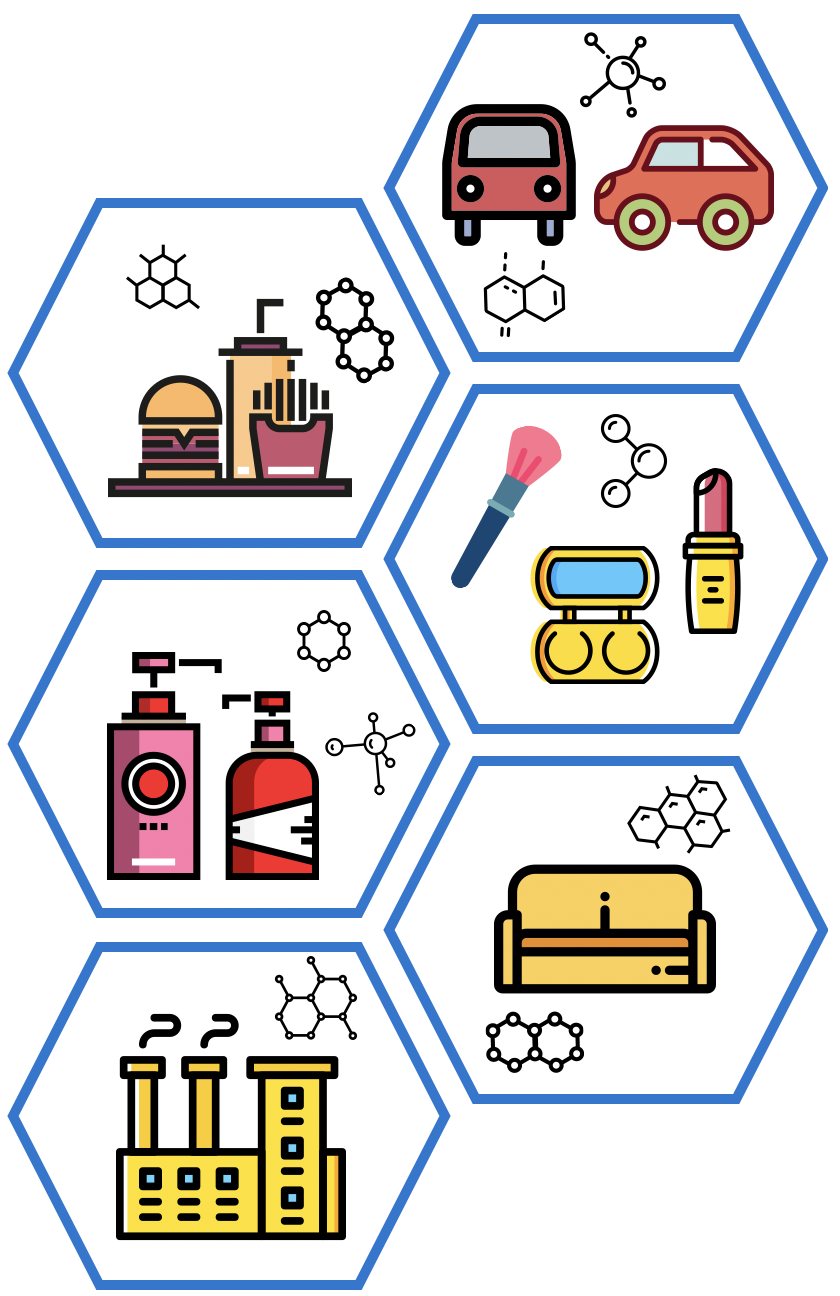
\includegraphics[scale=0.32]{figures/Screen Shot 2021-05-19 at 6.51.52 PM.png} \\
\end{center}
\end{columns}
}

\frame
{\frametitle{ Why care about environmental mixtures? }
\begin{columns}
\column{0.5\textwidth}
\vspace{2ex} \\
    {\begin{itemize}
        \item We are exposed to hundreds (thousands?) of chemicals at any single time point
        \pause
        \item Traditionally, epi studies have focused on single-chemical analyses
        \begin{itemize}
            \item This does not represent reality
        \end{itemize}
        \pause
        \item The {\color{matbluedark} combination} of exposures likely induces different responses 
    \end{itemize}}
\column{0.5\textwidth}
\begin{center}
\begin{changemargin}{-1.5em}{-1em}
	\onslide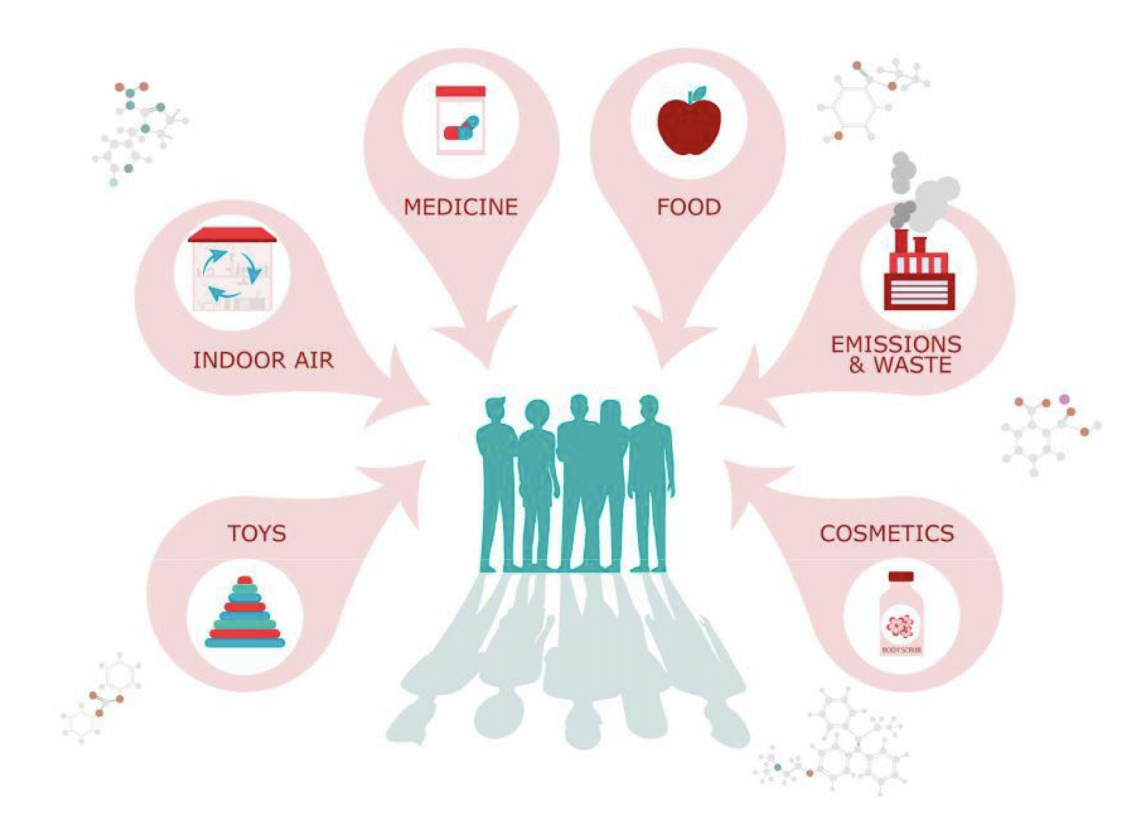
\includegraphics[scale=0.325]{figures/europa_image.png} \\
\end{changemargin}
\vspace{-1em}
\raggedleft
{\tiny\color{hgray}European Union, 2018}
\end{center}
\end{columns}
}

\frame[c]{
\frametitle{Endocrine disrupting chemicals as a mixture}
\begin{columns}
\column{.45\textwidth}
\vspace{1em}
\begin{changemargin}{-1em}{0em}
\begin{itemize}
    \item Defined by biological mechanism
    \pause
    \item Interfere with hormonal systems
    \pause
    \item Disrupt processes critical for brain development
    \vspace{1em}
    \pause
    \item Ubiquitous environmental exposure
    \begin{itemize}
        \item Consumer products
        \item Industrial products
    \end{itemize}
    \pause
    \item Often highly correlated
\end{itemize}
\end{changemargin}
\column{.55\textwidth}
\begin{changemargin}{-1em}{0em}
\onslide
\begin{center}
{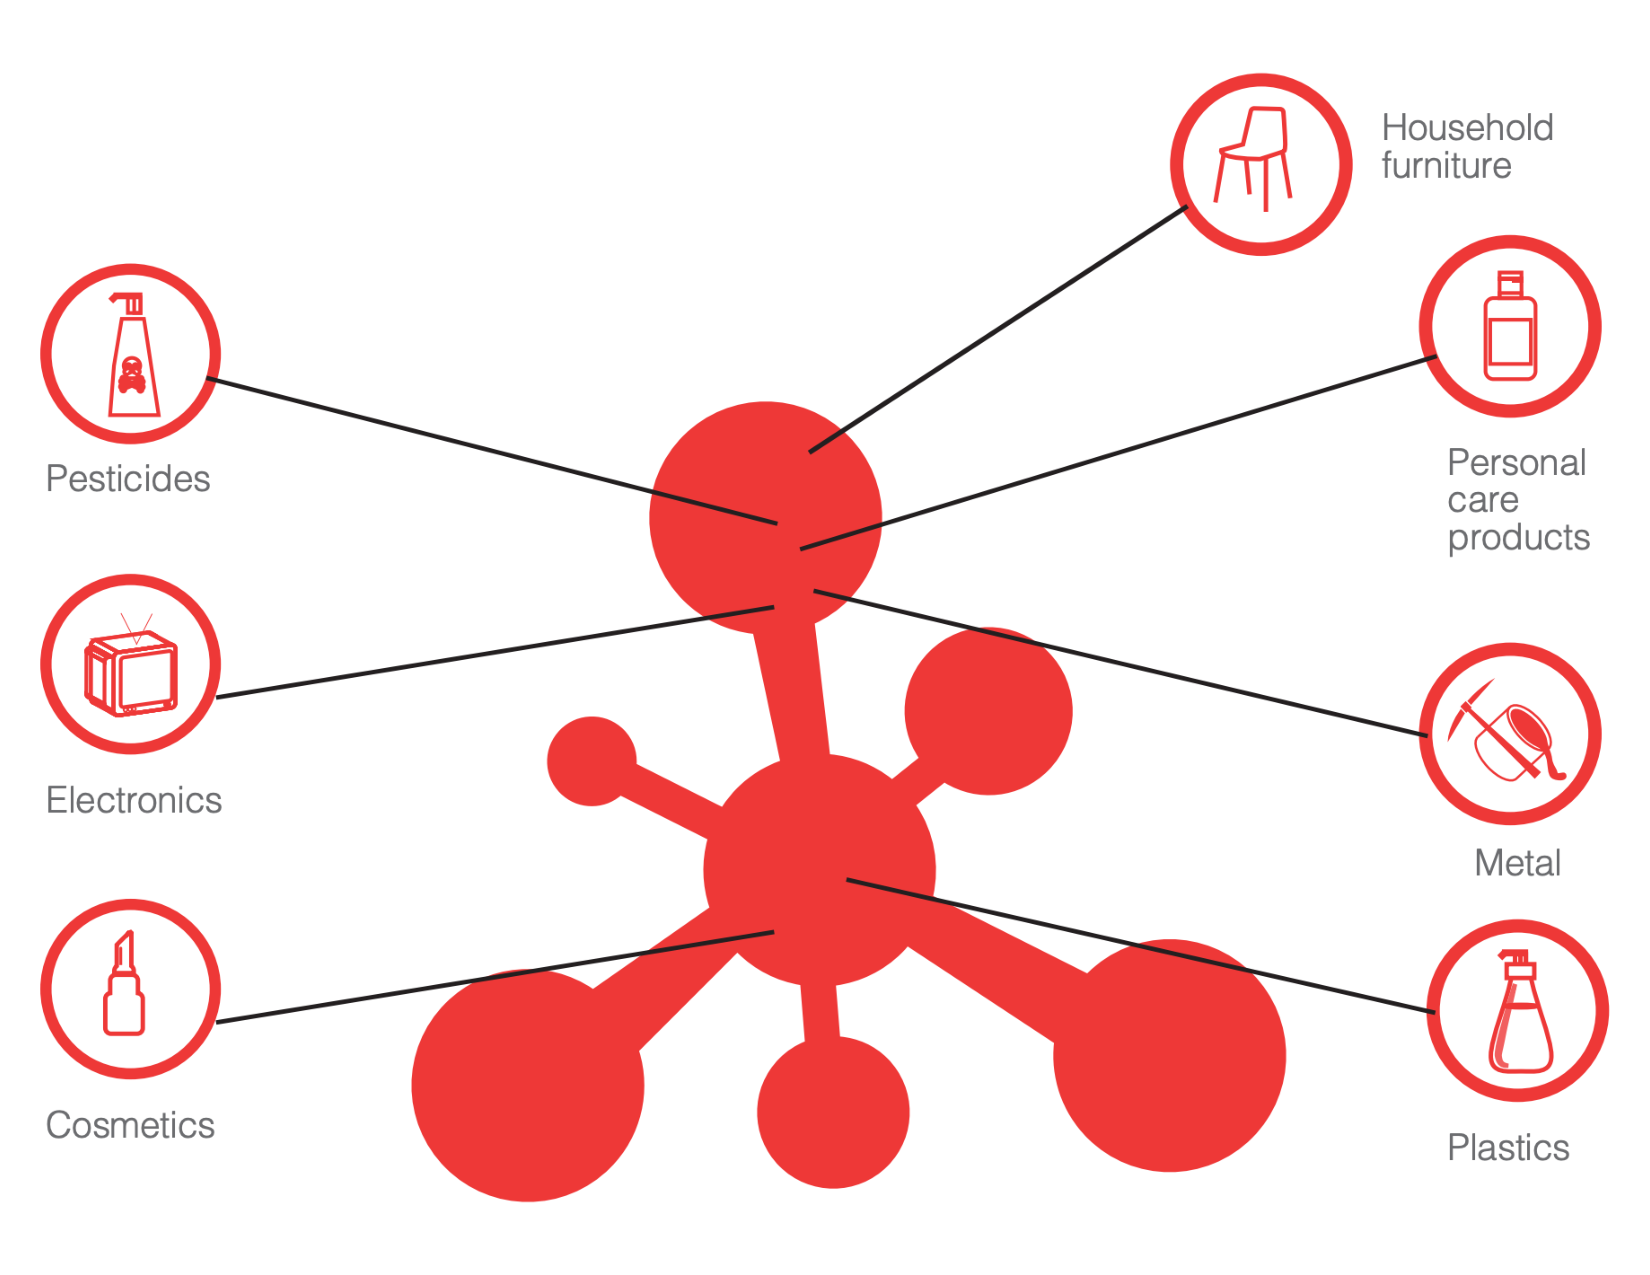
\includegraphics[scale = 0.23]{figures/un_edc.pdf}}
\end{center}
\vspace{-0.5ex}
\begin{flushright}
\tiny{\color{hgray}{U.N. Environmental Programme, 2017}}\phantom{x}
\end{flushright}
\end{changemargin}
\end{columns}
}

\frame{
\frametitle{Potential questions in mixtures analyses}

    \begin{columns}
	\column{0.4\textwidth}
    	\begin{tcolorbox}[boxrule=2pt,colframe=matbluedark, colback=white]
    		\centering
    		For mixtures analyses the appropriate method depends on the primary research question
	    \end{tcolorbox} 
	
	\column{0.6\textwidth}
	\vspace{2ex}
	    \begin{tikzpicture}[mindmap, grow cyclic,scale=0.8]
\begin{scope}[mindmap, concept color = white, text = matbluedark,
        	level 1 concept/.append style = {level distance = 92, sibling angle = 72}]
\node [concept, text = matbluedark, scale = 0.55] at (0,0) (pattern) {{\huge Mixtures Research Questions}} [clockwise from = 15]
        	child [concept color = matbluedark] {node [concept, text = white, scale = 0.7] (med) {{\large Overall Effect Estimation}}}
        	child [concept color = matbluedark] {node [concept, text = white, scale = 0.7] (med) {{\large Pattern Recognition}}} 
        	child [concept color = matbluedark] {node [concept, text = white, scale = 0.7] (med) {{\large Inter- actions}}} 
        	child [concept color = matbluedark] {node [concept, text = white, scale = 0.7] (med) {{\large {\it A priori} Defined Groups}}} 
        	child [concept color = matbluedark] {node [concept, text = white, scale = 0.7] (med) {{\large Toxic Agent Identification}}} ;
\end{scope}
\end{tikzpicture}	
\end{columns}
}

\frame{
	\frametitle{Exposure pattern recognition}
	\begin{columns}
		\column{0.4\textwidth}
		\begin{changemargin}{0em}{-2em}
		\begin{itemize}
			\item Why should we care about identifying {\color{matbluedark}exposure patterns} to chemicals in a population?
			\begin{itemize}
				\item Sources
				\item Behaviors
			\end{itemize}
			\pause
			\item If we link these patterns to (multiple) adverse health outcomes
			\begin{itemize}
				\item Efficient regulations
				\item Targeted interventions
			\end{itemize}
		\end{itemize}
		\end{changemargin}
		\column{0.6\textwidth}
			\vspace{2ex}
			\begin{changemargin}{0em}{-1em}
			\onslide
\begin{tikzpicture}[mindmap, grow cyclic,scale=0.8]
\begin{scope}[mindmap, concept color = white, text = matbluedark,
        	level 1 concept/.append style = {level distance = 92, sibling angle = 72}]
\node [concept, text = matbluedark, scale = 0.55] at (0,0) (pattern) {{\huge Mixtures Research Questions}} [clockwise from = 15]
        	child [concept color = matbluelight] {node [concept, text = white, scale = 0.7] (med) {{\large Overall Effect Estimation}}}
        	child [concept color = matbluedark] {node [concept, text = white, scale = 0.7] (med) {{\large Pattern Recognition}}} 
        	child [concept color = matbluelight] {node [concept, text = white, scale = 0.7] (med) {{\large Inter- actions}}} 
        	child [concept color = matbluelight] {node [concept, text = white, scale = 0.7] (med) {{\large {\it A priori} Defined Groups}}} 
        	child [concept color = matbluelight] {node [concept, text = white, scale = 0.7] (med) {{\large Toxic Agent Identification}}} ;
\end{scope}
\end{tikzpicture}
\end{changemargin}
\end{columns}
}

% \frame{
% 	\frametitle{Potential pattern recognition questions}
% \begin{columns}
% \column{0.55\textwidth}
% \begin{itemize}
%     \item Are there subgroups with similar exposure profiles?
%     \item Are certain combinations of exposure harmful?
%     \item 
% \end{itemize}
% \column{0.4\textwidth}
% \begin{center}
% 	\includesvg[scale=0.15]{figures/question-svgrepo-com.svg}
% 	\hspace{1ex} \includesvg[scale=0.15]{figures/question-svgrepo-com.svg} \\
% 	\vspace{1ex}
% 	\includesvg[scale=0.15]{figures/question-svgrepo-com.svg}
% 	\hspace{1ex} \includesvg[scale=0.15]{figures/question-svgrepo-com.svg} \\
% 	\vspace{1ex}	\includesvg[scale=0.15]{figures/question-svgrepo-com.svg}
% 	\hspace{1ex} \includesvg[scale=0.15]{figures/question-svgrepo-com.svg} \\
% \end{center}
% \end{columns}
% }

\frame{
	\frametitle{Limitations of existing exposure pattern recognition methods}
\begin{columns}
		\column{0.55\textwidth}
        \begin{itemize}
         \item Choice of $k$ patterns
         \pause
         \item Outlying values
         \pause
         \item Chemicals $<$ LOD
         \pause
         \item $+/-$ solution 
         \pause
         \item Orthogonality constraint
         \pause
         \item No measure of uncertainty
        \end{itemize}
        \pause
\vspace{1em}
\centering$\Longrightarrow$ Proposed solutions: \\
\vspace{1ex}
{\tt\color{matbluedark}\textbf{Principal component pursuit \&}} \\
{\tt\color{matbluedark}\textbf{Bayesian non-parametric non-negative matrix factorization}}
\column{0.5\textwidth}
\ \\
\vspace{1em}
\onslide
\begin{tikzpicture}[mindmap, grow cyclic,scale=0.5]
		\begin{scope}[mindmap, concept color = matbluedark, text = white, 
		level 1 concept/.append style = {level distance = 125, sibling angle = 90},
		level 2 concept/.append style = {level distance = 95, sibling angle = 50}]
		\node [concept, text = white, scale = 0.45] at (5,-3) (pattern) {{\LARGE Pattern Recognition}} [clockwise from = 50]
		child {node [concept, text = white, scale = 0.6] (med) {{\large Clustering}} [clockwise from=45]
			child [concept color = matbluelight] {node [concept, scale = 0.55] {\large K-means}}
			child [concept color = matbluelight] {node [concept, scale = 0.55] {\large Hierarchical}}}
		child {node [concept, text = white, scale = 0.6] (gen) {{\large Dimension Reduction}}
			child [concept color = matbluelight] {node [concept, scale = 0.55] {\Large PCA}}
			child [concept color = matbluelight] {node [concept, scale = 0.55] {Factor Analysis}}
			child [concept color = matbluelight] {node [concept, scale = 0.55] {\Large NMF}}};
		\end{scope}
 		\end{tikzpicture}	
{\scriptsize{\color{hgray}{$\ \hspace{3em} ^{\star}$Not an exhaustive list of methods!}}}
\end{columns}
}


% \frame{
% 	\frametitle{Comparing results across methods}
% 	\begin{itemize}
% 		\item Generally a good practice
% 		\begin{itemize}
% 			\item Especially if complementary methods 
% 			\item Sensitivity analyses to assess robustness of results  
% 		\end{itemize}
% 		\item If different methods address different questions, consistency in findings is welcome, but not expected
% 		\item If/when differences across methods are detected $\rightarrow$ keep in mind what the aim of each method is!
% 		\item Trying different methods and choosing the answer we like the best should {\it always} be avoided
% 		\begin{itemize}
% 			\item I.e., no cherry-picking!
% 		\end{itemize}
% 	\end{itemize}
% }


% \frame{
% \frametitle{Million dollar question}
%     \begin{itemize}
% 	    \item The necessity to assess exposure to mixtures is now well-recognized
% 	    \item US EPA, NRC, and NIEHS all agree 
%     \end{itemize}	
% \pause
% \vspace{5ex}
%     \begin{tcolorbox}[colframe=matbluedark, colback=white]
% 	    \centering
% 	    {\color{matbluedark}How} can we represent the compexity of reality in a (single) statistical model? 	
%     \end{tcolorbox}
% }

% \frame{\frametitle{ How do we deal with exposure to mixtures? }
%     \begin{itemize}
%         \item This is still a very open question
%         \item Existing methods have limitations
%         \item There have been several workshops held by EPA and NIEHS to address this issue
%         \item The most recent NIEHS workshop (2015) concluded that 
%         \begin{enumerate}
%             \item Although some methods performed better than others, the presented estimated associations were still quite variable and not in agreement
%             \item {\color{matbluedark}The choice of method should depend on the research question}
%     \end{enumerate}
%     \end{itemize}
% }

% \frame{\frametitle{Why do traditional methods fail?}
%     \begin{itemize}
%             \item Chemicals are often {\color{matbluedark}highly-correlated}
%             \begin{itemize}
%                 \item This means that they cannot go in the same regression model
%                 \item[$\Rightarrow$] Large standard errors and unstable effect estimates
%             \end{itemize}
%             \item Requires more flexible models
%             \begin{itemize}
%                 \item Group chemicals or assays
%                 \item Drop some chemicals
%                 \item Incorporate {\tt \color{matbluedark} machine learning techniques}
%             \end{itemize}
%     \end{itemize}
% }

% \frame{
% \frametitle{Some considerations}\
%     \begin{enumerate}
%         \item No single method outperforms all others for all potential questions
%         \item {\color{matbluedark} Interpretability}
%         \item {\color{matbluedark} Robustness} (stable solutions)
%         \item Computational scalability -- as $N$ and/or $p$ increase, some methods begin to fail
%         \item Exploration vs. hypothesis testing
%         \item Not a good idea to ``blindly'' use methods from other fields -- may need to adjust them first
%     \end{enumerate}
% }